\documentclass[10pt,journal,compsoc]{IEEEtran}
\usepackage{xeCJK}
\usepackage{amsmath}
\usepackage{mathtools}
\usepackage{amssymb}
\usepackage{float}

% *** CITATION PACKAGES ***
%
\ifCLASSOPTIONcompsoc
  % IEEE Computer Society needs nocompress option
  % requires cite.sty v4.0 or later (November 2003)
  \usepackage[nocompress]{cite}
\else
  % normal IEEE
  \usepackage{cite}
\fi

\begin{document}

\title{网络游戏中收集物品的概率问题}

\author{15211068~谭伟豪~~15211063~于牧之}

\maketitle

\newtheorem{definition}{Definition}
\renewcommand{\abstractname}{摘 要}
\renewcommand{\figurename}{图}
\renewcommand{\tablename}{表}
\renewcommand{\IEEEkeywordsname}{关键词}
\begin{abstract}

  网络游戏常需要玩家收集物品, 而很多时候玩家获得的物品是随机的. 同时, 玩家的目标也较为复杂. 我们对游戏中的收集要素进行了数学建模, 从而定量考察了游戏中的收集要素, 以帮助玩家更好地了解自己所玩的游戏.

\end{abstract}
\renewcommand{\abstractname}{Abstract}
\begin{abstract}
  Collecting elemnts often enter online games. In some of the games, the item that you get every time is random. Players 
\end{abstract}

\begin{IEEEkeywords}
概率, 收集式卡牌游戏.
\end{IEEEkeywords}
\renewcommand{\IEEEkeywordsname}{Keywords}
\begin{IEEEkeywords}
Probability, Collectible Card Game.
\end{IEEEkeywords}

\section{引言}

  目前市面上的网络游戏大多带有收集要素, 如地下城与勇士(DNF)中需要收集装备来提高自己的战斗力, 阴阳师中需要收集式神来优化自己的出战阵容. 对于这些游戏, 收集往往是一切的基础, 玩家只有收集到足够的物品才能体验游戏的全部内容.

  但是在这些游戏中, 玩家每次获得的物品往往是随机的. 如卡牌类游戏(CCG)中开卡包得到的卡, 大型多人在线角色扮演游戏(MMORPG)中从怪物身上获得的装备, 它们就像抽扑克牌一样具有随机性. 在这种随机性面前, 玩家往往将自己个人的所获所得归结为运气, 但从来没有对这类收集任务有一个整体的把握.由于这种强烈的随机性几乎只有在人为设计出来的游戏中才会被体会到,所以人们在日常生活中并没有积累到相关的经验,所以对于第一次进入游戏的新手,整个游戏的随机系统尤其具有迷惑性。事实上, 游戏中的收集任务远比在生活中收集东西要复杂, 人为设计出来的规则使得完成任务更加的困难。

  为了对搜集类游戏有一个清晰的认识,客观科学地评估其完成难度,从而能够更加理性地投入时间和金钱。地下城与勇士这款游戏中的装备获取过程是一个较为典型的搜集过程,我们决定以这款游戏为一个典型代表来分析网络游戏中收集物品的概率问题。

\section{DNF中的装备收集问题1}

  \subsection{问题描述}
    地下城与勇士中存在形形色色的装备, 在当前版本中, 总共有104件最高级别的装备, 玩家只能随机获得这些装备. 而玩家身上总共有12个装备槽, 因此完美获得所有装备就意味着玩家要获取这12个部位上最合适的装备.

    于是我们提出了这样的一个问题, 玩家获得了n件装备, 每件装备都等可能地取自容量为N的装备池. 玩家想凑齐其中指定的M件装备, 求凑齐的概率P与获得装备的数量n之间的关系.

  \subsection{模型假设}
    \begin{enumerate}
      \item 每件装备的获取概率是均等的
      \item 每次装备的获取是独立的
    \end{enumerate}

  \subsection{模型建立}
    概率等于所有事件中的某些事件在所有事件中所占的比率, 所以凑齐的概率就是凑齐的事件在所有事件中所占的比率. 我们可以得到
    \begin{align}
      P(\text{M件全齐}) &= 1-P(\text{M件中至少缺1件})\\
      &= 1-\frac{\text{至少缺1件的有序出装方案数}}{N^n}\\
      &= 1-\frac{\sum_{k=1}^{k=M}(-1)^k\binom{M}{k}(N-k)^n}{N^n}\\
      &= \frac{\sum_{k=0}^{k=M}(-1)^k\binom{M}{k}(N-k)^n}{N^n}
    \end{align}
    
    其中第(2)步到第(3)步应用了容斥原理, 具体推导如下.
    
    \begin{equation*}
      \begin{split}
        &~~~~~\text{至少缺1件的有序出装方案数} \\
        =&~~~~~\text{至少缺装备1的有序出装方案数} \\
        &+ \text{至少缺装备2的有序出装方案数} \\
        &+ \cdots \\
        &+ \text{至少缺装备M的有序出装方案数} \\
        &- \text{至少缺装备1, 装备2的有序出装方案数} \\
        &- \text{至少缺装备1, 装备3的有序出装方案数} \\
        &- \cdots \\
        &- \text{至少缺装备M-1, M的有序出装方案数} \\
        &+ \text{至少缺装备1, 2, 3的有序出装方案数} \\
        &+ \cdots \\
        &\cdots
      \end{split}
    \end{equation*}

    综上
    $$
    P(\text{M件全齐})=\frac{\sum_{k=0}^{k=M}(-1)^k\binom{M}{k}(N-k)^n}{N^n}
    $$

  \subsection{求解}
    代入问题描述中的实际数据, 即N=104, M=12, 得到凑齐概率P与获得装备的数量n之间的关系如图\ref{fig:solution1}所示

    \begin{figure*}[!ht]
    \centering
    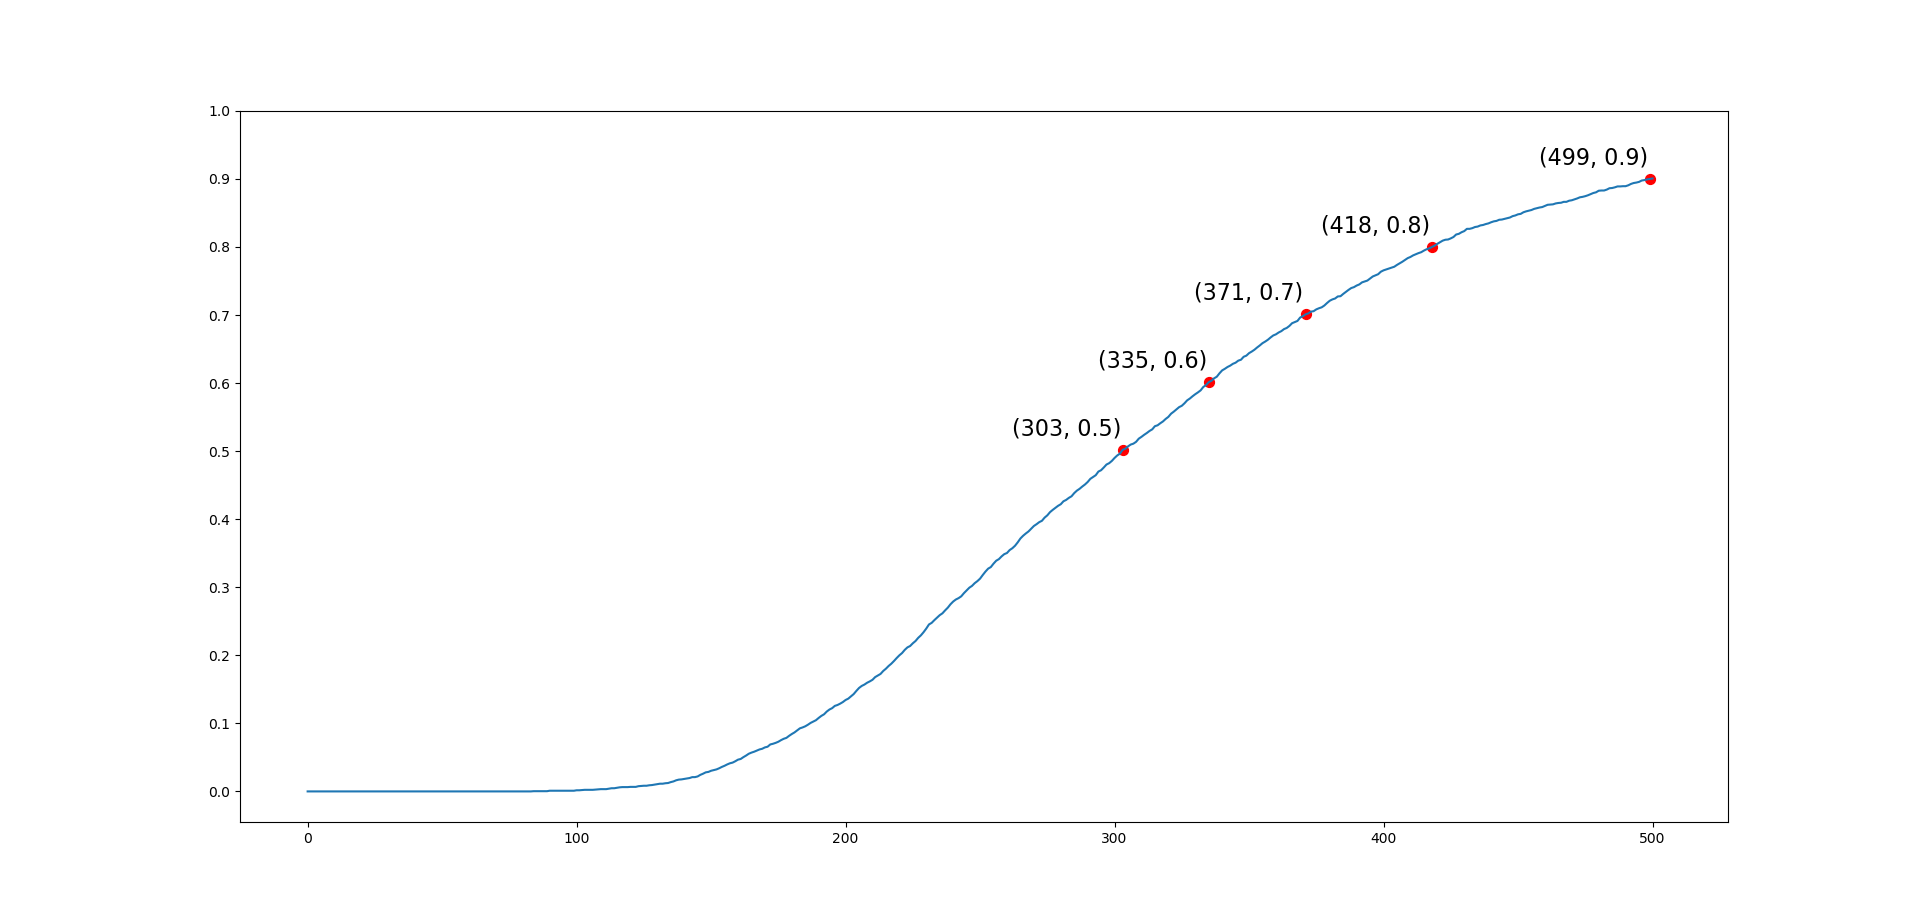
\includegraphics[width=30pc]{img/solution1.png}
    \caption{DNF中的装备收集问题1}
    \label{fig:solution1}
    \end{figure*}


\section{DNF中的装备收集问题2}
  我们已经通过容斥原理得到了一个正确的模型,但是仔细想来,这个模型并不能很好地解决实际游戏过程中的装备毕业问题。在地下城与勇士这款游戏中,一个部位的装备往往有多件强度较高的装备可供选择,例如剑士既可以使用太刀作为武器也可以使用巨剑,每个职业都有布甲、皮甲、轻甲、重甲和板甲5中类型的护甲装备可供选择。而且游戏中还存在着装备套装的概念,3件或者5件特定装备组合成为套装,拥有强大的套装属性。在地下城与勇士现阶段的游戏中,布甲、皮甲、轻甲、重甲和板甲各有一套套装作为终极毕业装备。虽然这5套套装属性之间各有差异,但是大多数玩家都认为获得其中的任意1套或者是获得这5套之中指定2套或者3套之中的任意1套就算是装备毕业,而不是获得像是在模型中讨论的一样非要得到指定的一套套装或者是武器才能够毕业。所以我们的模型需要进行修改。

  \subsection{定义}

  在修改我们的模型之前,我们将先定义一些游戏中类似收集任务的基本概念, 以便后续讨论. 
  
  物品I (Item): 游戏中可获得的基本单元.

  物品组G (Group): 物品构成的集合, 为游戏中发挥作用的组合单元.
  
  候选项集C (Candidate Group): 物品组构成的集合, 物品组即其中的候选项. 对于一个候选项集, 我们只需要获得其中的一个物品组即可满足收集目标. 
  

  集合的展开 (Flatten): 将嵌套的集合展开. 其递归定义为
  $
  flatten(S) = \left\{
    \begin{aligned}
      & \bigcup\limits_{E \in S} flatten(E) &, S~is~a~set \\
      & \{E\} &, otherwise
    \end{aligned}
  \right.
  $

  目标的完成: 对于目标集$T = \{C_1, C_2, \dots, C_n\}$和已收集的物品集合$S$, 目标的完成当且仅当
  $ \exists P = \{G_{k_1}, G_{k_2}, \dots, G_{k_n} | G_{k_i} \in C_i\}, s.t. flatten(P) \subseteq S$
  
  \vspace{5mm}

  \subsection{问题描述}
  使用上述的定义,我们可以较为简洁地给出地下城与勇士中有多种选择的收集问题案例描述:
  
  物品: $I_1$=皮甲肩甲, $I_2$=皮甲上衣, $I_3$=皮甲裤子, $I_4$=皮甲腰带, $I_5$=皮甲鞋子, $I_6$=轻甲肩甲, $I_7$=轻甲上衣, $I_8$=轻甲裤子, $I_9$=轻甲腰带, $I_{10}$=轻甲鞋子, $I_{11}$=太刀, $I_{12}$=巨剑, $I_{13}$=手镯, $I_{14}$=项链, $I_{15}$=戒指, $I_{16}$=辅助装备, $I_{17}$=魔法石, $I_{18}$=耳环, $I_{19},I_{20}...I_{104}$=所有非目标装备(游戏中总共有104件装备). 
  
  物品组: 皮甲套$G_1=\{I_1, I_2, I_3, I_4, I_5\}$, 轻甲套$G_2=\{I_6, I_7, I_8, I_9, I_{10}\}$, 太刀$G_3=\{I_{11}\}$, 巨剑$G_4=\{I_{12}\}$, 首饰套$G_5=\{I_{13}, I_{14}, I_{15}\}$, 辅助装备$G_6=\{I_{16}\}$, 魔法石$G_7=\{I_{17}\}$, 耳环$G_8=\{I_{18}\}$.

  候选项集: 衣服$C_1=\{G_1, G_2\}$, 武器$C_2=\{G_3, G_4\}$, 首饰$C_3=\{G_5\}$, 辅助装备$C_4=\{G_6\}$, 魔法石$C_5=\{G_7\}$, 耳环$C_6=\{G_8\}$

  目标集: $T=\{C_1, C_2, C_3, C_4, C_5, C_6\}$

  

  目标的完成:获得了皮甲套和轻甲套之一, 太刀和巨剑之一, 首饰套, 辅助装备, 魔法石, 耳环.即$P=\{G_{1}, G_{3}, G_{5}, G_{6}, G_{7}, G_{8}\}$或$\{G_{1}, G_{4}, G_{5}, G_{6}, G_{7}, G_{8}\}$或$\{G_{2}, G_{3}, G_{5}, G_{6}, G_{7}, G_{8}\}$或$\{G_{2}, G_{4}, G_{5}, G_{6}, G_{7}, G_{8}\}$


  \subsection{模型的建立}
  假设在一共有n件物品,目标集一共有$m = card(flatten(T))$个,即目标获得的物品为m个,获得的k个物品中有s个属于$flatten(T)$,即获得了我们想要的s个物品,我们可以发现只要$s>min(card(flatten(P)))$,即s不小于完成目标所需要的物品数的最小值,那么均有可能达成目标.所以所有这些情况的可能达到目标的概率之和即为目标完成的概率。 
  
  之前得到的模型的推倒较为复杂,要想计算获得的k个物品中有s个是我们想要的物品十分的繁琐,使得其计算有候选项集的问题时效率较低。我们发现当我们在目标集中拥有s个物品时,之后的状态如在目标集中拥有s+1个物品仅仅与拥有s个物品时的状态有关,与s-1和再之前的状态都没有关系,所以该问题的随机过程具有马尔科夫性,这个过程是一个马尔科夫过程,于是我们可以马尔科夫链的性质来解决该问题。

  我们用状态s表示已经获得了目标集中的s个物品,状态s仅有保持原状态,和向状态s+1转移这两种转移方式。在计算状态转移时的概率时,我们做了一个简化,认为所有物品获得的概率是相同的,事实情况也确实大多如此。那么状态s转移到状态s+1的概率是$\frac{m-s}{n}$,而保持原状态的概率是$1-\frac{m-s}{n}$。于是我们可以得到状态转移矩阵T(如表1 空白的地方用0填补)。

  \begin{table*}[]
    \centering
    \caption{状态转移矩阵}
    \label{tab:markov}
    \begin{tabular}{c|cccccccccc}
        & 0 & 1 & 2 & 3 & ... & s & s+1 & ... & m-1 & m \\ \hline
    0   & $1-\frac{m}{n}$ & $\frac{m}{n}$ &   &   &     &   &     &     &     &   \\
    1   &   & $1-\frac{m-1}{n}$ & $\frac{m-1}{n}$ &   &     &   &     &     &     &   \\
    2   &   &   & $1-\frac{m-2}{n}$ & $\frac{m-2}{n}$ &     &   &     &     &     &   \\
    ... &   &   &   &   &     &   &     &     &     &   \\
    s   &   &   &   &   &     & $1-\frac{m-s}{n}$ & $\frac{m-s}{n}$ &     &     &   \\
    ... &   &   &   &   &     &   &     &     &     &   \\
    m-1 &   &   &   &   &     &   &     &     &  $1-\frac{1}{n}$  & $\frac{1}{n}$ \\
    m   &   &   &   &   &     &   &     &     &     &  $1$
    \end{tabular}
  \end{table*}

  \begin{figure*}[!ht]
    \centering
    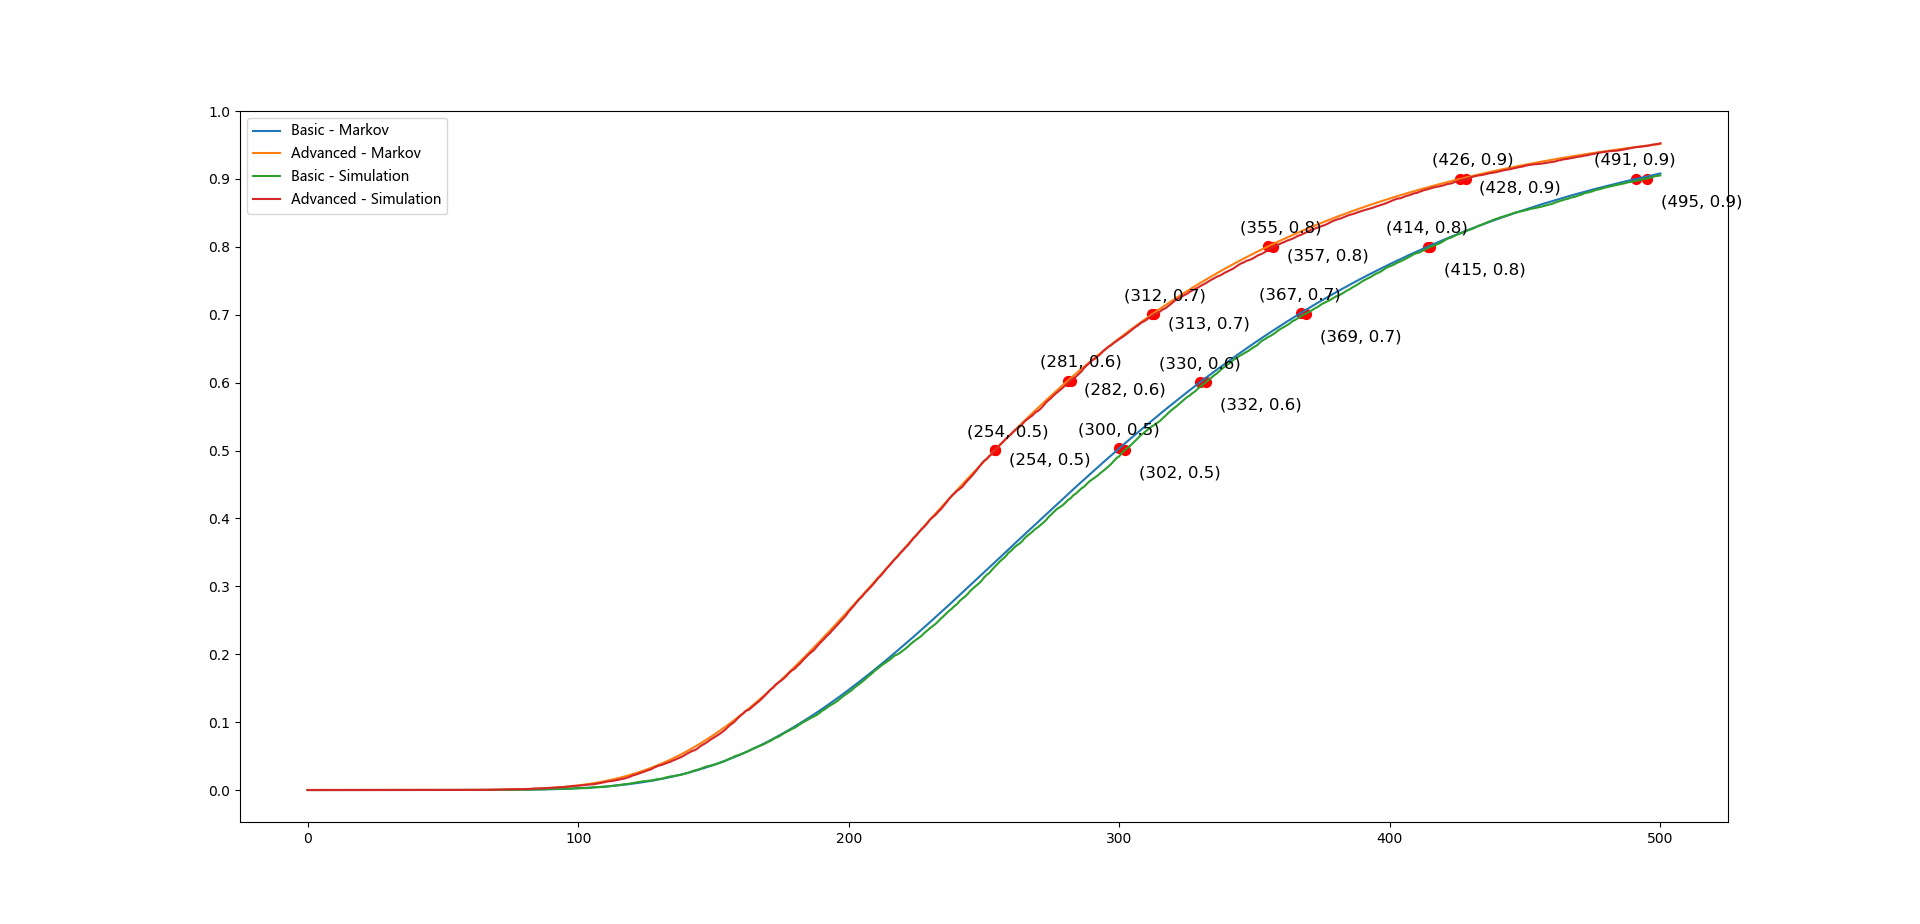
\includegraphics[width=45pc]{img/everything_about_dnf.png}
    \caption{DNF收集完成概率理论计算与程序模拟对比图, 其中Basic曲线描述的是收集问题1, Advanced曲线描述的是收集问题2, 横坐标代表获取装备此数, 纵坐标代表完成收集目标的概率(理论)/频率(模拟)}
    \label{fig:dnf_comprehensive}
  \end{figure*}
  
  获得k个物品后,经过了k次状态转移,得到获得物品的概率分布情况$\{1,0,0,...,0\}*T^k$

  知晓了获得物品的概率分布情况之后,接下来便是要计算在获得k个物品的情况中,完成目标的概率是多少。这个时候,由于这k个物品所组成的集合可能包含多个候选项集,候选项集之间又存在交叉,所以我们需要再次使用容斥原理来解决这个问题。
  
  $$
  P(\bigcup_{i=1}^n A_i) = \sum\limits_{k=1}^n (-1)^{k-1} \sum_{\substack{I \subset \{ 1,\dots, n \}\\ |I|=k}} P(A_I)
  $$
  
  在我们的问题中, 若记已收集集合为$S$, 对于目标集$T$, 定义事件$A_j = flatten(\{G_{k_1}, G_{k_2}, \dots, G_{k_n} | G_{k_i} \in C_i, i = 1,\dots,|T|\}) \subset S$, 其中$j=\overline{k_1 k_2 \dots k_n}$
  
  则当获得m件装备时完成收集目标的概率为
  \begin{equation*}
    \begin{split}
      & P(\bigcup_{i=1}^n A_i) \\
      = & \sum\limits_{k=1}^n (-1)^{k-1} \sum_{\substack{I \subset \{ 1,\dots, n \}\\ |I|=k}} P(P_I\subset S)\\
      = & \sum\limits_{k=1}^n (-1)^{k-1} \sum_{\substack{I \subset \{ 1,\dots, n \}\\ |I|=k \\ m \geq P_I}} \frac{\binom{|P_I|}{|P_I|} \binom{n-|P_I|}{m-|P_I|}}{\binom{n}{m}}
    \end{split}
  \end{equation*}

  \subsection{模型的验证}
<<<<<<< HEAD
    地下城与勇士的装备获取是可以用程序模拟的. 我们模拟了3000名玩家, 统计了完成收集任务的玩家占总玩家数的比重, 并将这个数据与数学推导的结果进行了比较, 结果如图\ref{fig:dnf_comprehensive}


  \subsection{结论}
    我们可以看到程序模拟出的结果与我们用模型计算得出的结果高度吻合,证明了我们建模的正确性。同时我们也可以看到,尽管达成目标的途径变为了4倍,但是为了完成目标所需要获得的物品数缺只是减少了15\%左右,从这个角度来看,可以看出地下城与勇士的耐玩程度和毕业通关的困难程度。
=======
    地下城与勇士的装备获取是可以用程序模拟的. 我们模拟了3000名玩家, 统计了完成收集任务的玩家占总玩家数的比重, 并将这个数据与数学推导的结果进行了比较, 结果如图\ref{fig:dnf_comprehensive}所示. 
>>>>>>> 532e29100cf7bb82af3cacf630685a4bc81ecb14
    
    


\section{阴阳师中的抽卡问题}
为了证明我们建立的模型具有较为广泛的适用性,我们决定另选一款游戏来测试我们的模型。相较于地下城与勇士中装备爆率与毕业问题来说,阴阳师是更加典型的抽卡游戏,更能够简介明了地反映我们的模型。阴阳师是完全基于式神养成的游戏,而游戏中的核心——式神的获得全部来自于抽卡,式神的等级分为SSR、SR、R、N,其中SSR最为稀有也最为强大,是所有玩家的终极追求。

\subsection{问题描述}
某刘姓玩家经过长时间的努力,终于只剩下2个SSR没有获得了,他为了集齐所有的SSR实现一直以来苦苦追求的目标积攒了1000次抽卡的机会,已知每次抽卡都有1\%的几率抽到一张随机的SSR,阴阳师目前一共有18个不同的SSR,请问刘同学有多大的概率能够实现它的目标呢?

\subsection{模型的建立}
<<<<<<< HEAD
直接套用上面推倒出的马尔科夫链模型即可得出结论,我们可以看到该同学只有不到20\%的可能性能够抽到剩下的两个他所没有的SSR达成目标,如图\ref{fig:yys1k}所示. 那么我们再来看看到底要多少抽才能比较有把握地达成目标呢?图\ref{fig:yys1w}告诉我们一共需要4000多抽,该同学才能有80\%的较大把握达成搜集齐所有SSR的目标。
=======
直接套用上面推导出的马尔科夫链模型即可得出结论,我们可以看到该同学只有不到20\%的可能性能够抽到剩下的两个他所没有的SSR达成目标,如图\ref{fig:yys1k}所示. 那么我们再来看看到底要多少抽才能比较有把握地达成目标呢?图\ref{fig:yys1w}告诉我们一共需要4000多抽,该同学才能有80\%的较大把握达成搜集齐所有SSR的目标。
>>>>>>> 532e29100cf7bb82af3cacf630685a4bc81ecb14

\begin{figure}[H]
  \centering
  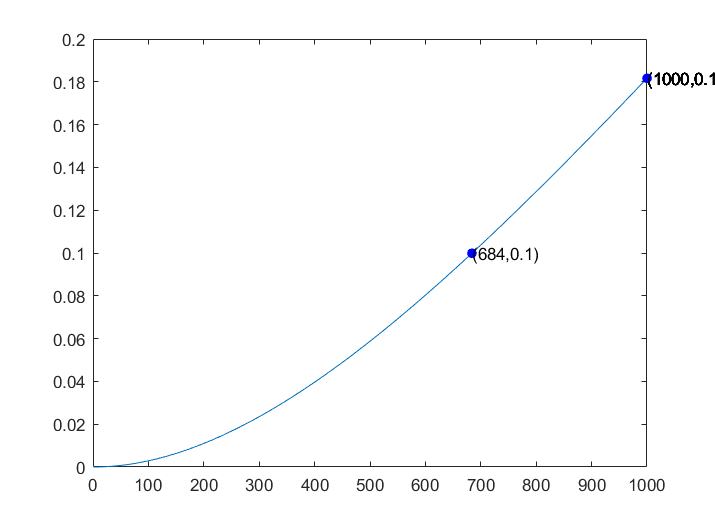
\includegraphics[width=20pc]{img/yys1k.png}
  \caption{阴阳师一千抽概率图}
  \label{fig:yys1k}
\end{figure}

\begin{figure}[H]
  \centering
  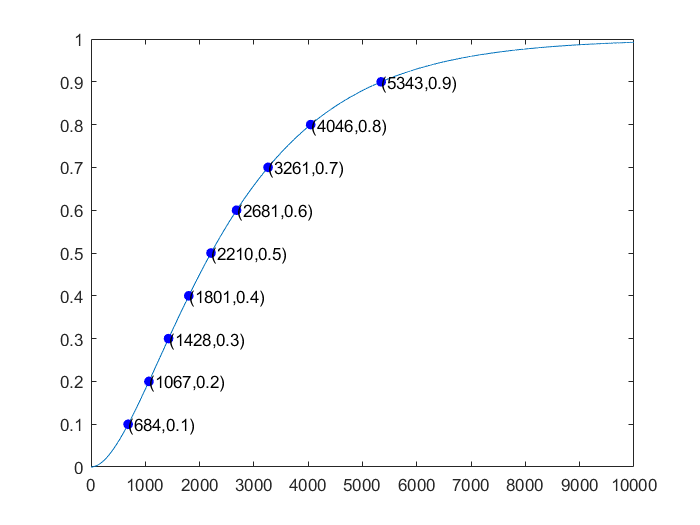
\includegraphics[width=20pc]{img/yys1w.png}
  \caption{阴阳师一万抽概率图}
  \label{fig:yys1w}
\end{figure}


\section{结论}



\bibliographystyle{IEEEtran}
\bibliography{thesis}

\end{document}
